\section{CV template}
% This is unique for class presentation.
\newcommand{\where}{in the facebook event.}
\begin{frame}{\LaTeX CV-template}{Can be found \where}
    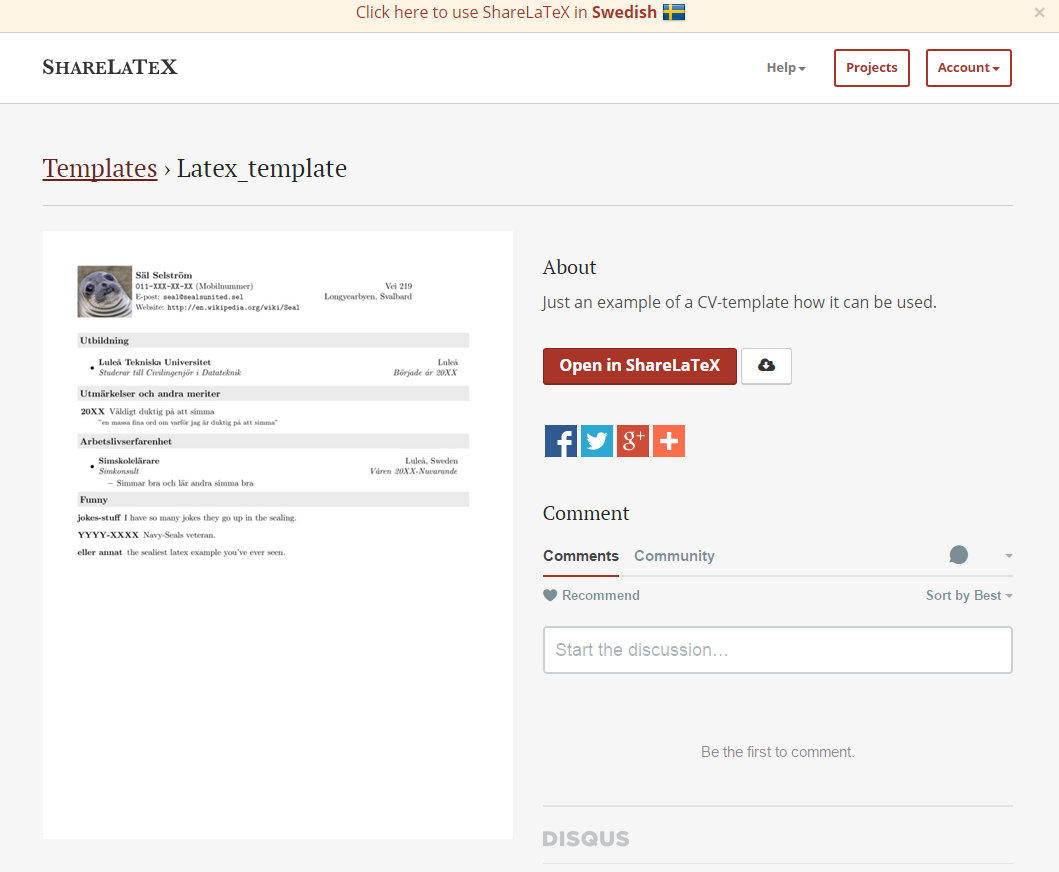
\includegraphics[width=\textwidth]{img/2-cvlatex.png}
\end{frame}

\begin{frame}{\LaTeX CV-template}{Can be found \where}
    Take some time and download the template. \\ \ \\ \ \\
    \small This link also works: \\ \ \\ \ \\
    \normalsize
    \texttt{http://tinyurl.com/ddoslatex}
\end{frame}

\begin{frame}{\LaTeX CV-template}
	Things to notice: \\ \ 
	\begin{itemize}
	\item \textbackslash newcommand
	\item \textbackslash minipage
	\end{itemize} 
\end{frame}

\subsection{Newcommand}
\begin{frame}[fragile]{Defining your own commands}
	\begin{block}{A way of defining new commands}
	\begin{lstlisting}
	\newcommand{\command}{something}
	\end{lstlisting}
		When calling \textbackslash command, we would get: 
		\begin{lstlisting}
		<@\textcolor{blue}{something}@>
		\end{lstlisting}
	\end{block}
   	\begin{block}{With arguments}
   		\begin{lstlisting}
		\newcommand{\command}[1]{something #1}
		\end{lstlisting}
		When calling \textbackslash command[seal], we would get:	
		\begin{lstlisting}
		something seal
		\end{lstlisting}
   \end{block}
\end{frame}

\begin{frame}[fragile]{Commands calling other commands}
	\begin{block}{A command calling another command}
	   	\begin{lstlisting}
		\newcommand{\fstcmd}[1][]{cmd1 #1 \sndcmd[#1]}
		\newcommand{\sndcmd}[1][]{cmd2 #1}
		\end{lstlisting}
		When calling \textbackslash fstcmd[seal], we would get: 
		\begin{lstlisting}
		<@\fstcmd[seal]@>
		\end{lstlisting}
   \end{block}
\end{frame}

\subsection{Minipage}
\begin{frame}[fragile]{A page in a page}
	\begin{block}{Acts like boxes.}
	\begin{lstlisting}
		\begin{minipage}[pos][height][contentpos]{width}
	\end{lstlisting}
   \end{block}
\end{frame}

\begin{frame}{Minipage}{Split pages?}
    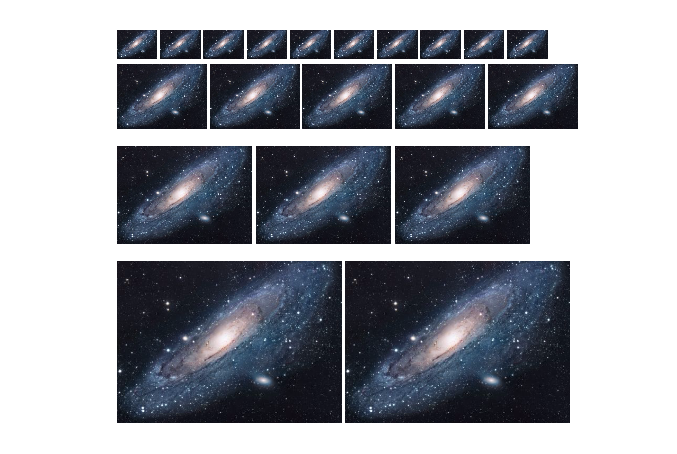
\includegraphics[width=\textwidth]{img/2-minipage.png}
\end{frame}

\begin{frame}[fragile]{Minipage - Continued}{\textbackslash begin\{minipage\}[pos][height][contentpos]\{width\}}
   more reading:
   \begin{lstlisting}
   http://en.wikibooks.org/wiki/LaTeX/Boxes#minipage_and_parbox
   http://www.sascha-frank.com/latex-minipage.html
   \end{lstlisting}
\end{frame}